%% Please fill in your name and collaboration statement here.
\newcommand{\studentName}{**FILL IN YOUR NAME HERE**}
\newcommand{\collaborationStatement}{**FILL IN YOUR COLLABORATION STATEMENT HERE \\ (See the syllabus for information)**}


%%%%%%%%%%%%%%%%%%%%%%%%%%%%%%%%%%%%%%%%%%%%%%%
\documentclass[solution, letterpaper]{cs20}
\usepackage{enumerate}
\usepackage{tikz}
\usepackage{pgf}
\usepackage{tikz}
\usepackage{hyperref}
\begin{document}
\header{2}{Due Wednesday, February 19, 2016 at 9:59am. All students should submit an electronic copy.}


%%%%%%%%%%%%%%%%%%%%%%%%%%%%%%%%%%%%%%%%%%%%%%%
\PART{Jack}
%%%%%%%%%%%%%%%%%%%%%%%%%%%%%%%%%%%%%%%%%%%%%%%

\problem{3+3+4+4}{3 lines each}

\subproblem Put the following formula in conjunctive normal form: $(p \leftrightarrow q) \land r$
\subproblem Put the following formula in disjunctive normal form: $(p \oplus q) \rightarrow (r \land q)$
\subproblem Put the following formula in disjunctive normal form: $((p \rightarrow q) \rightarrow p) \rightarrow p$. When is this formula satisfied?
\subproblem Prove that any propositional formula can be written in disjunctive normal form. 

\begin{solution}
\subsolution  We can replace $p \leftrightarrow q$ with $(p \rightarrow q) \land (q \rightarrow p)$. The statement then becomes $(p \rightarrow q) \land (q \rightarrow p) \land r$, which we can rewrite as $(\lnot p \lor q) \land (\lnot q \lor p) \land r$, which is in CNF.

\subsolution Recall that $p \oplus q \equiv (p \lor q) \land \lnot (p \land q)$. The expression then expands to $(p \lor q) \land \lnot (p \land q) \rightarrow (r \land q)$ which is equivalent to $\lnot((p \lor q) \land \lnot (p \land q)) \lor (r \land q)$. Using De Morgan's laws to remove the negation, we get $\lnot (p \lor q) \lor (p \land q) \lor (r \land q)$, which simplifies to $(\lnot p \land \lnot q) \lor (p \land q) \lor (r \land q)$.

\subsolution Eliminating $\rightarrow$, we get $\lnot (\lnot (\lnot p \lor q) \lor p) \lor p$. Then, pushing the negations inwards, the expression becomes $(\lnot (\lnot p \lor q) \land \lnot p) \lor p$ and $((\lnot p \lor q) \land \lnot p) \lor p$. Finally, pushing the disjunctions in using the distributive property gives $(\lnot p \lor q \lor p) \land (\lnot p \lor p)$. This is a tautology, known as Peirce's law.

\subsolution A statement is in DNF if it is the or of ands. For any expression, we can generate a truth table for every possible combination of inputs. We can convert the rows of this table that evaluate to true to a statement in DNF. To do so, for each line that evaluates to true, create a clause that "ands" together the variables turned on in that line. If any one of these individual clauses evaluates to true, the whole expression will evaluate to true. Thus, the final expression in DNF is all of these clauses "or-ed". 

\end{solution}

%%%%%%%%%%%%%%%%%%%%%%%%%%%%%%%%%%%%%%%%%%%%%%%
\PART{Michelle}
%%%%%%%%%%%%%%%%%%%%%%%%%%%%%%%%%%%%%%%%%%%%%%%

\problem{2+2}{1/3 page}

While wandering the halls of Hogwarts, Harry stumbles upon a note that reads: "Danger lies before you, while safety lies behind. Drink some of us to help you, the combination you must find". Harry sees four bottles of mysterious potion, one colored red, one blue, one yellow, and one green. A sign next to the door reads:

\begin{enumerate}
\item Drink two of these potions, one must be colored blue.
\item If blue you do not have, the other three will tide you through.
\item Pair not blue with red
\item Or face your fate with dread
\end{enumerate}

Luckily, Harry sees all the colored bottles. Define r, y, b, g:
\begin{enumerate}
\item r: Harry drinks the red potion
\item y: Harry drinks the yellow potion
\item b: Harry drinks the blue potion
\item g: Harry drinks the green potion
\end{enumerate}

\subproblem Write a proposition that evaluates to True if Harry selects a valid combination of potions. 
\subproblem Draw a logic circuit that implements the proposition in (a) with as few gates as possible from this list: \textsc{Not}, \textsc{Or}, \textsc{And}, \textsc{Xor}, \textsc{Nand}, \textsc{Xnor}. Feel free to draw a picture of the circuit and include a photograph in your LaTex file. 

\begin{solution}

\subsolution $(r \land y \land g) \lor (b \land (y \oplus g))$

could also do 
$(r \land y \land g) \lor (b \land y) \lor (b \land g)$
\subsolution 
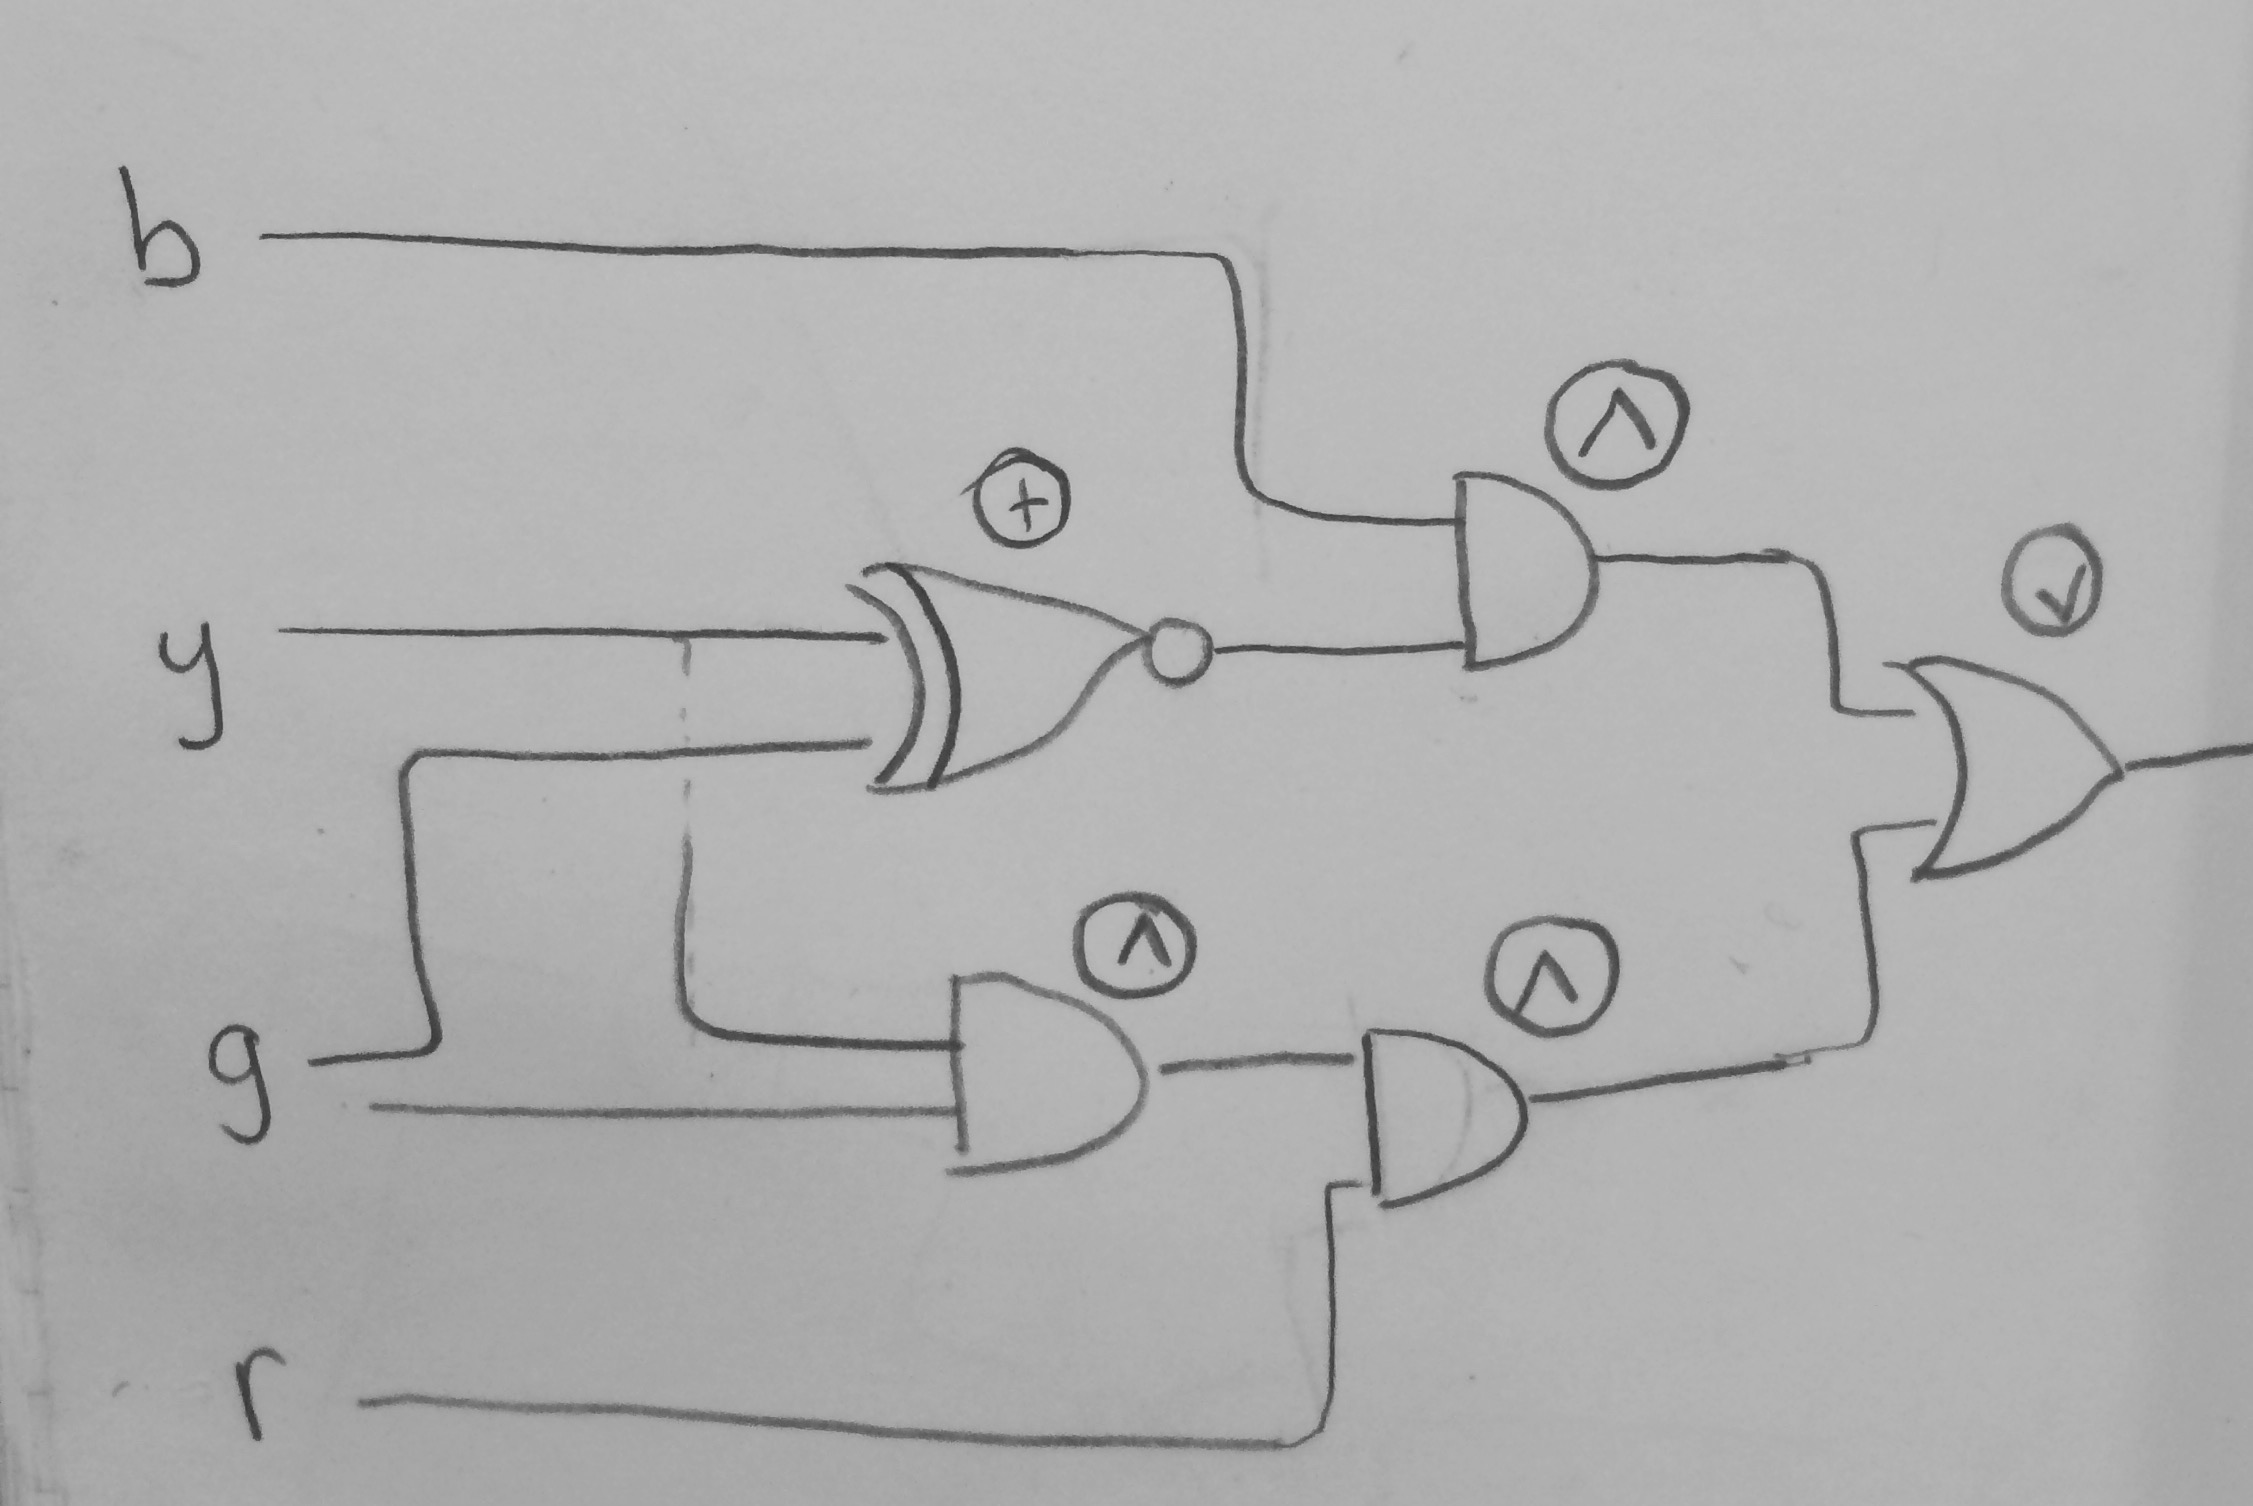
\includegraphics[width=3in]{LogicGate.jpg}

\end{solution}

\problem{3+3+2}{1/2 page}

The Boolean function $G(p,q,r)$ is defined in the table. You can think of the table as a truth table where the last column is the value of some unknown compound proposition consisting of the variables p, q, and r. Additionally, ``0'' represents False and ``1'' represents True. 


\begin{table}[h]
\centering

\begin{tabular}{| c c c | c |}
\hline
p & q & r & G(p,q,r) \\ \hline
0 & 0 & 0 & 0 \\ 
0 & 0 & 1 & 0 \\ 
0 & 1 & 0 & 0 \\ 
0 & 1 & 1 & 1 \\ 
1 & 0 & 0 & 0 \\ 
1 & 0 & 1 & 1 \\ 
1 & 1 & 0 & 0 \\ 
1 & 1 & 1 & 0 \\ \hline

\end{tabular}
\end{table}

\subproblem Construct a proposition in disjunctive normal form whose value is the last column of the truth table. 
\subproblem Show that the proposition in (a) is equivalent to $(p \oplus q)\land r$ using the properties of identies.
\subproblem How many logic gates would be required to construct a circuit for the expression in (a), assuming you didn't simplify it? How many for the simplified expression in (b)?  In both cases, you may use any types of logic gates you wish. No justification required, just a number. 

\begin{solution}

\subsolution
Writing one term for each row in which $G(p, q, r)$ is true, we conclude:
$$G(p, q, r) \equiv (\lnot p \land q \land r) \lor (p \land \lnot q \land r)$$

\subsolution
Using the identity $p \oplus q \equiv (p \land \lnot q) \lor (\lnot p \land q)$, we can write:
  \begin{align*}
      (p \oplus q) \land r & \equiv ((p \land \lnot q) \lor (\lnot p \land q)) \land r \\
                           & \equiv (p \land \lnot q \land r) \lor (\lnot p \land q \land r) \\
                           & \equiv (\lnot p \land q \land r) \lor (p \land \lnot q \land r)
  \end{align*}
\emph{Note:  This problem can also be solved by showing that the two expressions have the same truth table.}

\subsolution
For the expression in (a), you would need 1 \textsc{Or}, 2 \textsc{Not} and 4 \textsc{And} gates, for a total of 7 logic gates.
For the expression in (b), you would need 2 logic gates, 1 \textsc{And} and 1 \textsc{Xor}.

\end{solution}

\end{document}
